\chapter{Metody}
V následující sekci je popsán formát vstupních souborů vytvořeného programu a kni\-hov\-ny použité v rámci implementace. Zmíněn je  též externí nástroj MACH, kterým byla pro klasifikované molekulové sady provedena a vyhodnocena parametrizace vybraných empirických metod. 

\section{Structure-Data file (SDF)}
Formát SDF \cite{sdf_pdf, sdf_clanek} patří s formáty Molfile, RGfile, rxnfile, RDfile a XDfile mezi CTfile formáty (\textit{Chemical Table file})  vyvinuté pro reprezentaci chemických dat. SDF je rozšířením formátu Molfile (zkr. MOL). 
%Narozdíl od formátu MOL umožňuje SDF zápis více záznamů do jednoho souboru. 
Umožňuje zápis více záznamů do jednoho souboru, přičemž každý záznam ukončený sekvencí '\verb|$$$$|' reprezentuje jednu molekulu. 

Záznamy v SDF souboru mají pevně danou strukturu, odvozenou od struktury MOL souborů. Společnými  částmi záznamu obou formátů jsou tzv. \textit{header block} a tzv. \textit{connection table} (viz obr. x). % K vlozenemu obrazku dat komentar, ze to je struktura spolecna pro SDF a MOL ze vlastnosti v properties block v SDF nejsou
V~SDF záznamu mohou být narozdíl od formátu MOL za řádek '\verb|M END|' připojeny specifikace biologických či fyzikálně-che\-mic\-kých vlastností dané molekuly. 
% Základní pravidla pro tvorbu SDF záznamů jsou následující

Struktura SDF záznamů je následující:
\begin{itemize}
    \item \textit{Header block} se skládá ze tří řádků obsahujících název molekuly, datum vytvoření záznamu, program použitý pro generování záznamu a komentář. 
    %První řádek obsahuje název molekuly, na druhém řádku jsou vyhrazeny indexy pro datum vytvoření záznamu, program použitý pro generování záznamu, dimenzi souřadnic atomů atd. Třetí řádek obsahuje komentář. 
    Všechny tři řádky mohou být prázdné.
    \item \textit{Counts line} obsahuje na definovaných indexech řádku počet atomů a vazeb  popsaných v sekcích \textit{Atom block} a \textit{Bond block}, informaci o chiralitě molekuly a verzi molekulového záznamu (V2000 nebo V3000).
    \item \textit{Atom block} obsahuje souřadnice atomů  $x, y, z$ a symbol prvku. Další indexy řád\-ků, ve většině případů obsazené symbolem '\verb|0|', slouží pro bližší specifikaci vlastností atomů. Na základě pořadí atomů v \textit{Atom block}u jsou v sekci \textit{Bond block} specifikováni vazební partneři a typ vytvořené vazby. 
    \item \textit{Data items} slouží pro doplňující záznamy vlastností molekuly. Řádek \textit{Data header}, začínající znakem \verb|'>'|, obsahuje název dané vlastnosti nebo identifikační číslo molekuly v databázi MACCS-II. Následují řádky s příslušnými hodnotami.
    %(např. \verb|'<melting.point>'|)
\end{itemize}

\section{PDB formát}
Formát PDB (\textit{Protein Data Bank}) je molekulový formát vyvinutý pro počítačovou reprezentaci biologicky aktivních makromolekul. Existuje ve dvou verzích, v původní verzi 2.0 a v novější verzi 3.0. V PDB souboru jsou obsaženy informace o prostorovém uspořádání molekuly, strukturní faktory pro rentgenovou krystalografii a data z NMR experimentu. PDB formát je v současnosti nahrazován standardizovaným formátem mmCIF.

PDB formát nese kromě dat o prostorovém uspořádání struktury informace o primární a sekundární struktuře nukleových kyselin a proteinů. Informace ohledně 3D struktury nesou záznamy (tj. řádky PDB souboru) začínající sekvencí 'ATOM'. Tyto záznamy obsahují na definovaných pozicích sériové číslo atomu, zkratku residua, jemuž atom přísluší, \textit{x}, \textit{y} a \textit{z} souřadnice, symbol prvku apod. Záznamy 'HETATM' označují nestandardní residua (např. ligandy nebo kofaktory enzymů) a mají stejnou strukturu jako záznamy 'ATOM'. Záznamy 'HELIX' a 'SHEET' popisují sekundární strukturu proteinů. 'SSBOND' je záznam vyhrazený pro specifikaci disulfidických můstků mezi cysteinovými residui \cite{PDB1, PDB2}. 

\subsection{Nomenklatura atomových typů aminokyselin}
PDB soubory používají pro specifikaci atomů proteinogenních aminokyselin atomové typy deklarované nomenklaturou IUPAC \cite{AA_nomenclature}. Tato nomenklatura označuje atomy vedlejšího řetězce aminokyseliny dle vzdálenosti od uhlíku s navázanou karboxylovou skupinou a aminoskupinou. Řecká písmena v označení atomů (C$^\alpha$, C$^\beta$, C$^\gamma$, C$^\delta$, C$^\varepsilon$, C$^\zeta$, C$^\eta$) jsou v nomenklatuře nahrazena velkými písmeny latinské abecedy (CA, CB, CG, CD, CE, CZ, CH). Pro specifické atomy aminokyselin (vodík navázaný na C$^\alpha$, kyslík COO$^-$ skupiny hydrolyzovaný při tvorbě peptidické páteře) jsou definovány speciální atomové typy (HA, OXT), atomy aromatických jader však nejsou odlišeny. Mezi verzemi 2.0 a 3.0 PDB formátu došlo ke změně názvů vybraných atomových typů, popsaná nomenklatura tak není napříč PDB soubory plně konzistentní. 

\begin{figure}[h]
\begin{center}
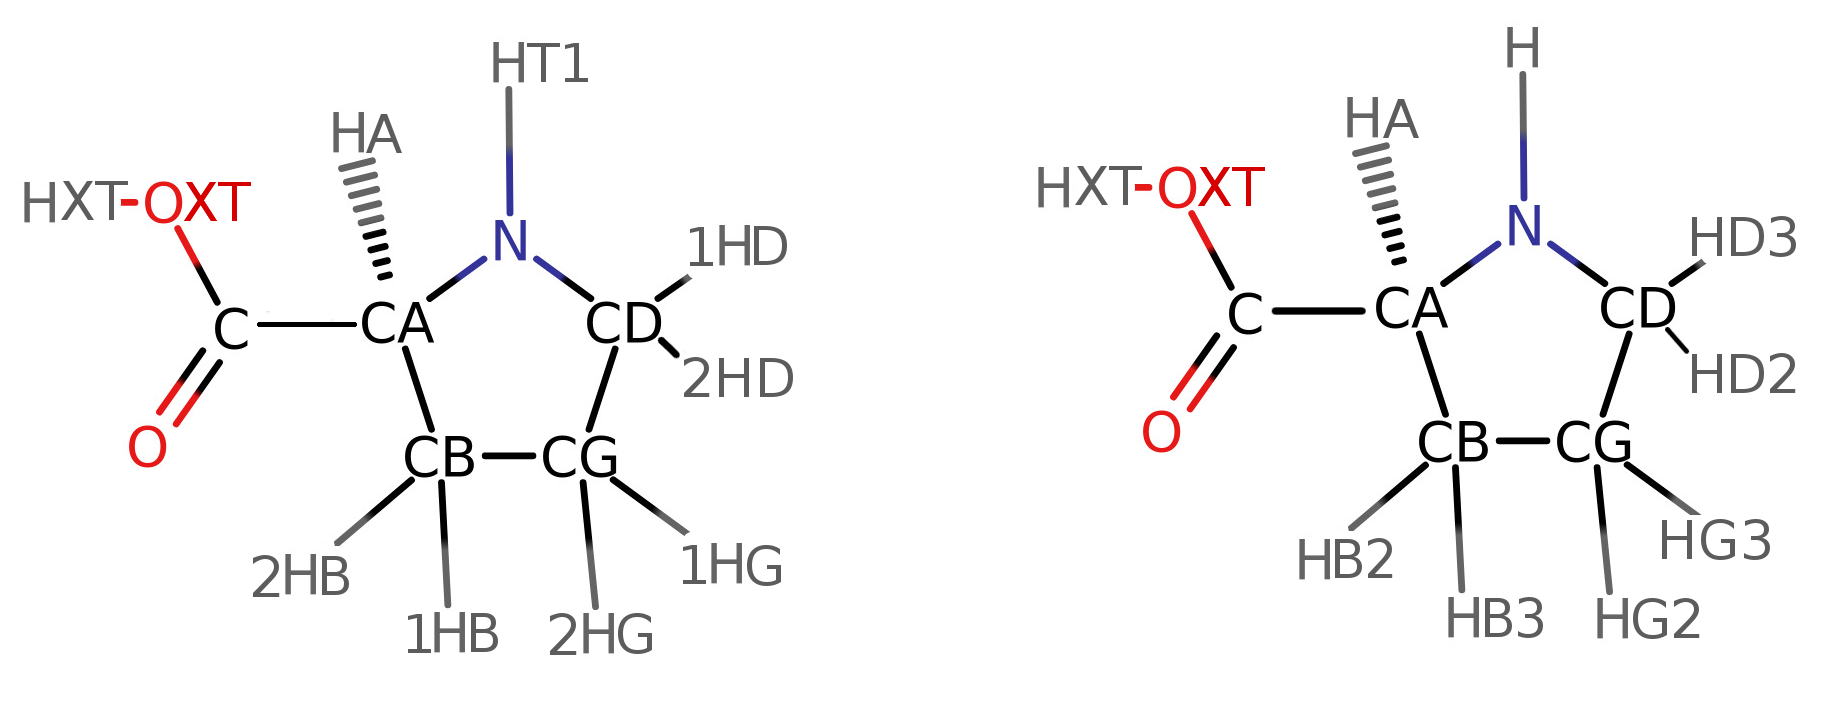
\includegraphics[width=12cm]{pictures/prolin_merged.png}
\caption{Porovnání názvů atomových typů molekuly prolinu v jednotlivých verzích PDB formátu. Vlevo je zobrazena verze 2.0, vpravo verze 3.0. Změny v názvech atomů se týkají atomů vodíku.}
\end{center}
\end{figure}
% https://www.cgl.ucsf.edu/chimera/docs/UsersGuide/tutorials/pdbintro.html
% ftp://ftp.wwpdb.org/pub/pdb/doc/format_descriptions/Format_v33_Letter.pdf

\section{SMILES}
% zdroje: http://www.daylight.com/smiles/index.html; Leach - Chemoinformatics; Bunin- Chemoinformatics
SMILES \cite{Weininger, Bunin, Leach_chemo} (angl. \textit{Simplified Molecular Input Line Entry System}) je počítačová notace molekul či molekulových reakcí definovaná pomocí ASCII symbolů. SMILES reprezentace byla vyvinuta v 80. letech pro usnadnění práce s chemickými daty  a zvýšení efektivity jejich zpracování (např. prohledávání molekulových databází, vyhledávání podstruktur v molekulách). Zápis SMILES vychází z teorie grafů. Molekula je v~tomto kontextu chápána jako graf, tzn. uspořádaná dvojice množiny vrcholů a množiny hran $G(V,E)$. Průchodem molekulového grafu vzniká jednoznačný SMILES zápis molekuly, kde je každý vrchol (atom) a každá hrana (vazba) navštívena pouze jednou.

Základními prvky SMILES notace jsou symboly atomů a vazeb. Atomy jsou reprezentovány symbolem příslušného prvku. Pokud se jedná o atom aromatický, je pro jeho specifikaci použito malé písmeno (SMILES notace benzenu je '\verb|c1ccccc1|', cyklohexanu '\verb|C1CCCCC1|'
%benzen je pomocí SMILES notace zapsán jako \verb|'c1ccccc1'|, cyklohexan jako \verb|'C1CCCCC1'|
). Atomy vodíku jsou implicitně doplněny na základě valence základního stavu atomu, na který jsou navázány, a nemusí být  zadány explicitně. Pro~specifikaci počtu navázaných vodíků je třeba použít zápisu '\verb|[AHX]|', kde \verb|A| je symbol prvku a \verb|X| počet navázaných vodíků. Vazba jednoduchá, dvojná, trojná a aromatická jsou reprezentovány symboly '\verb|-|', '\verb|=|', '\verb|#|' a '\verb|:|'. Vazby jednoduché a aromatické nejsou ve většině SMILES výrazů explicitně zadány.

SMILES notace definuje zápis strukturních prvků sloučenin jako jsou cykly, větvení řetězců, chiralita a izomerie (E/Z a cis/trans izomerie). Přítomnost cyklu ve sloučenině indikují symboly atomů následované stejným číslem, viz např. výše uvedený SMILES pro benzen. Tyto atomy tvoří vazebný pár a cyklus tak uzavírají. Symboly atomů a vazeb uzavřené v kulatých závorkách značí vedlejší větve hlavního řetězce \cite{SMILES_exm}. 
%SMILES notace umožňuje také zápis chemických reakcí. 
% pod SMILES dat obrazek z Leache, pokud SMARTS budou dostatecne dlouhe, pokracovat s nimi pod obrazkem

\section{SMARTS}
\label{SMARTS}
SMARTS notace \cite{SMARTS_intro, SMARTS_exm} (angl. \textit{SMiles ARbitrary Target Specification}) je odvozena z notace SMILES, kterou rozšiřuje o další funkční prvky. Každý SMILES výraz je validním SMARTS výrazem, opačný přístup však vždy neplatí. Příčinou toho je fakt, že SMARTS je narozdíl od  notace SMILES, která slouží pro popis celých molekul, zaměřena na vyhledávání podstruktur. Validní SMARTS výraz '\verb|cOc|', popisující kyslík navázaný na dva aromatické uhlíky (můžeme najít např. v molekule difenyletheru), neodpovídá žádné reálné molekule, a není proto platným SMILES výrazem. 

SMARTS rozšiřuje SMILES notaci o užití logických operátorů. Symboly '\verb|&|' a '\verb|;|' značí logické \verb|AND|, přičemž symbol '\verb|&|' má vyšší prioritu v kombinaci s ostatními logickými operátory. Symbol '\verb|,|' značí logické \verb|OR|. Pro negaci výrazů je použit symbol '\verb|!|'. Užití jmenovaných logických operátorů je ilustrováno v tabulce \ref{logops} níže.

Dalším specifickým prvkem SMARTS výrazů je konstrukce  '\verb|$(XY)|', kde \verb|XY| reprezentuje platný SMARTS výraz. Touto konstrukcí lze snadno specifikovat atom v závislosti na jeho chemickém okolí. Příkladem je výraz '\verb|[O-;!$([O-]C(=O))]|', který definuje kyslíkový anion, jenž zároveň není součástí aniontu karboxylové skupiny COO$^-$. 
\begin{table}[h]
\label{logops}
\renewcommand{\arraystretch}{1.3}
    \begin{small}
    \hspace{7mm}\begin{tabular}{c|l}
        % \hline
        \verb|[c,n&H1]| & aromatický uhlík nebo (aromatický dusík s jedním vodíkem) \\
        \hline
        \verb|[c,n;H1]| & (aromatický uhlík nebo aromatický dusík) s jedním vodíkem \\
        \hline
        \verb|[!#6][O][H]| & hydroxylová skupina navázaná na jakýkoli atom kromě dusíku \\
        \hline
        \verb|[CX4,c][O][H]| & alkoholová skupina navázaná na alifatický či aromatický uhlík \\
        \hline
        \verb|[NX3;!$(NC=O)]| & trojvazný dusík, který není součástí amidové skupiny\\
        % \hline
    \end{tabular}
    \end{small}
    \caption{Příklad užití logických operátorů v notaci SMARTS. V pravém sloupci jsou popsány vyhledané strukturní motivy.}
\end{table}
\section{RDKit}
RDKit \cite{rdk_info} je volně dostupná open-source knihovna pro práci s chemickými daty, určena pro jazyky Java a Python. RDKit poskytuje standardní funkce pro zpracování chemických dat, jako je načítání široké škály molekulových formátů, práce s 2D a 3D reprezentací molekul, zápis molekulových reakcí, hledání strukturních motivů molekul a vizualizace výstupů. Kromě jmenovaných funkcí umožňuje propojení s PostgreSQL databází \cite{Postgre}. Základní datové struktury a algoritmy RDKitu jsou implementovány v jazyce C++, což v porovnání s interpretovaným jazykem Python zvyšuje jejich výkonnost.

\section{MACH}
MACH je software pro parametrizaci empirických metod výpočtu parciálních atomových nábojů (viz kap. Parametrizace \ref{param}) vyvinutý v rámci diplomové práce Bc. Ondřeje Schindlera v Národním centru pro výzkum biomolekul v Brně \cite{mach}. 

Software MACH byl vyvinut s cílem optimalizovat parametrizaci empirických metod výpočtu parciálních nábojů za použití optimalizační metody Guided Minimization \cite{guided_m}. Software je vyvinut v jazyce Python za využití specializovaných knihoven pro práci s vědeckými daty (SciPy \cite{scipy}, NLopt \cite{nlopt}). V softwaru byla úspešně implementována parametrizace empirických metod EEM, PEOE, SFKEEM \cite{sfkeem}, QEq \cite{molsimul}, ACKS2 \cite{acsk2} a MGC \cite{mgc}. Pro potřeby této bakalářské práce byly využity parametrizace prvních dvou jmenovaných metod. Kromě parametrizace MACH umožňuje výpočet parciálních nábojů molekul pomocí vybrané empirické metody, extrakci informací o vstupním SDF souboru či srovnání obsahu dvou nábojových sad.
